\section{Dominio abierto (Qanus/Freeling/CLEF)}

%%%%%%%%%%%%%%%%%%%%%%%%%%%%%%%%%%%
%%
%%			Introducción
%%
%%%%%%%%%%%%%%%%%%%%%%%%%%%%%%%%%%%
\subsection{Introducción}

\begin{frame}
\frametitle{Introducción}
  \begin{itemize}
    \item Sistema de dominio abierto multilingüe
    \item Basado en Qanus, adaptado para usar Freeling.
    \item Ejercicios de CLEF'07 monolingüe para español y portugués
    \item Wikipedia como base de conocimiento
  \end{itemize}

  Adoptamos el framework Qanus y el sistema QA-sys para:
  \begin{enumerate}
    \item Incorporar Freeling como librería de herramientas de procesamiento del lenguaje permitiendo un funcionamiento multilenguaje. 
    \item Trabajar sobre el corpus de datos y preguntas de los ejercicios de CLEF '07 de español y portugués
    \item Incorporamos y evaluamos algunas mejoras tomadas de la reseña a la literatura científica
  \end{enumerate}

\end{frame}

%%%%%%%%%%%%%%%%%%%%%%%%%%%%%%%%%%%
%%
%%			Marco teórico
%%
%%%%%%%%%%%%%%%%%%%%%%%%%%%%%%%%%%%
\subsection{Marco teórico}

\begin{frame}
\frametitle{Dominio de problemas y enfoque}
     \begin{block}{Dominio general y universal}<1->
      \begin{itemize}
          \item Cualquier cosa
          \item Corpora de texto $\rightarrow$ datos no estructurados
          \item Question answering como sistema de pipeline
          \item IR + NLP + Heurísticas
      \end{itemize}
    \end{block}
\end{frame}

\begin{frame}
\frametitle{Marco teórico}
  Consenso general sobre la arquitectura: pipeline de al menos 3 componentes:
  \begin{itemize}
    \item Módulo de procesamiento de la pregunta
    \begin{itemize}
      \item Submódulo principal: Question Classifier
      \item Anotaciones de la pregunta (NER, POS, QC, Otros: focus, answer type)
      \item Expansión/reformulación de la consulta (Heurística de Lampert, Moldovan)
    \end{itemize}
    \item Módulo de procesamiento de documentos
    \begin{itemize}
      \item Submódulo principal: índice invertido (estructuras de IR)
      \item (Otros: división en parágrafos, filtrado grueso, re-ranking)
    \end{itemize}
    \item Módulo de procesamiento de la respuesta
    \begin{itemize}
      \item Valor agregado ppal de un sistema de QA sobre uno de IR
      \item El menos estandarizado de los tres
      \item Heurísticas puntuales basadas en casos.
    \end{itemize}
  \end{itemize}

\end{frame}

\begin{frame}
\frametitle{Heurística de generación de queries [Lampert, 2004]}
\begin{block}{8 pasos}<1->
\begin{enumerate}
\item Palabras no stop words entre comillas
\item Entidades nombradas reconocidas
\item Construcciones nominales con sus adjetivos
\item Demás construcciones nominales
\item Sustantivos con sus adjetivos
\item Demás sustantivos
\item Verbos
\item El \sq{focus} de la pregunta
\end{enumerate}
\end{block}
\end{frame}

\begin{frame}
\frametitle{Competencias y métricas}
\begin{itemize}
\item {\color{red}FILL ME}
\end{itemize}
\end{frame}


%%%%%%%%%%%%%%%%%%%%%%%%%%%%%%%%%%%
%%
%%			Implementación
%%
%%%%%%%%%%%%%%%%%%%%%%%%%%%%%%%%%%%
\subsection{Implementación}

%%%%%%%%%%%%%%%%%%%%%%%%%%%%%%%%%%%
%%
%%      Ejercicio de Clef
%%
%%%%%%%%%%%%%%%%%%%%%%%%%%%%%%%%%%%
\subsubsection*{Ejercicios}

\begin{frame}
\frametitle{Ejercicios}
  \textit{Cross-Language Evaluation Forum}
  \begin{itemize}
    \item Principal organizador de conferencias de question answering multilingüe para idiomas europeos.
    \item La tarea principal de '07 presentaba una complejidad adecuada para el scope de esta tesis.
  \end{itemize}
  Ejercicios
  \begin{itemize}
    \item Subset de dos ejercicios de la tarea principal de question answering de '07. 
    \item Corpora, inputs de prueba y resultados esperados para una experimentación sobre diferentes idiomas disponible.
    \item Wikipedia + newsletters como corpus
    \begin{itemize}
      \item Nosotros trabajamos solo con las wikipedias
    \end{itemize}
    \item 200 preguntas (factoids, definition o list)
    \item Respuesta exacta. Topics + clusters + co-referencia.
    \item Preguntas sin respuesta
    \item Tomamos ejercicios monoligüe es-es y pt-pt (español-español y portugués-portugués)
  \end{itemize}
\end{frame}


\begin{frame}
  \frametitle{Tareas activadas en CLEF '07}
  \begin{figure}
      \includegraphics[scale=0.4]{graficos/clef07}
    \caption{Tareas activadas en la competencia Clef '07}
    \label{fig:tareas}
  \end{figure}
\end{frame}

\begin{frame}
\frametitle{Preguntas}
  \begin{center}
  \begin{table}
  \centering
  \begin{tabular}{| l | l | l | l | l | l |}
  \hline
  Subset & Idioma & Factoid & Definition & List & Total \\ \hline
  \multirow{2}{*}{Todo} & es & 158 & 32 & 10 & 200 \\ \cline{2-6}
   & pt & 159 & 31 & 10 & 200 \\ \hline
   \multirow{2}{*}{Wiki} & es & 130 & 24 & 9 & 163 \\ \cline{2-6}
   & pt & 104 & 18 & 8 & 130 \\ \hline
  \end{tabular}
  \caption{Totales por tipo de pregunta}
  \label{table:totals-type-question}
  \end{table}
  \end{center}

  Ejemplo de grupo con tema y correferencia (primer cluster de preguntas para es-es):
  \begin{itemize}
  \item ¿En qué colegio estudia Harry Potter?
  \item ¿Cuál es el lema del colegio?
  \item ¿En qué casas está dividido?
  \item ¿Quién es el director del colegio?
  \end{itemize}

\end{frame}


%%%%%%%%%%%%%%%%%%%%%%%%%%%%%%%%%%%
%%
%%      Sistema
%%
%%%%%%%%%%%%%%%%%%%%%%%%%%%%%%%%%%%
\subsubsection*{Sistema}

\begin{frame}
\frametitle{Qanus}
  \textit{Question-Answering @ National University of Singapore}
  \begin{itemize}
    \item Un framework de question answering basado en information retrieval
    \item QA-sys: un sistema de QA funcional simple construido sobre este framework. 
    \item Actualizado por última vez en noviembre de 2012, código abierto
    \item Herramientas de NLP de Stanford (POS, NER y QC, para inglés) y Lucene. 
    \item Estructura de Pipeline. Orientado para TREC 07 (Aquaint)
  \end{itemize}
\end{frame}

\begin{frame}
\frametitle{Qanus}
  \begin{figure}
      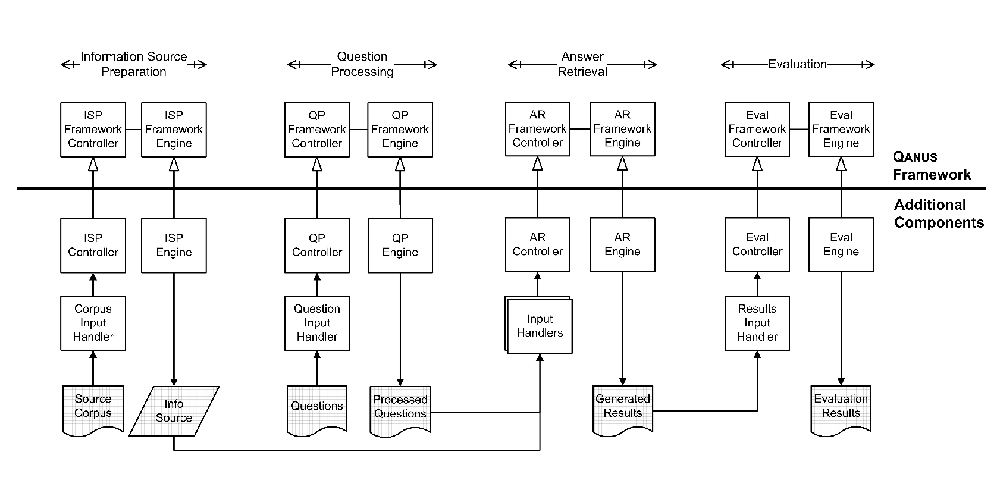
\includegraphics[scale=0.7]{graficos/Quanus}
    \caption{El framework Quanus y la implementación QA-sys}
    \label{fig:Quanus}
  \end{figure}
\end{frame}

\begin{frame}
\frametitle{El pipeline de QA-Sys}
  \textbf{1. Preparación de la fuente de información: } Preprocesa XML de Aquaint (datos de la TREC 07) de manera offline (llamado previo) en un índice Lucene \newline

\textbf{2. Análisis de la pregunta: } Anota la pregunta con POS, NER y QC. \newline

\textbf{3. Generación de respuestas: } Busca la pregunta en el índice, separa los documentos en pasajes y los rankea con métricas heurísticas y luego, dependiendo del tipo de QC, aplica heurísticas basadas en NER, POS y QC sobre los pasajes para extraer una respuesta\newline
  

  \begin{block}{QA-Sys}
    \begin{itemize}
      \item Compitió en TREC 07 con buenos resultados:
      \begin{itemize}
        \item  LymbaPA07 (privado)  $\rightarrow$ 0.706, 1ero
        \item Quanta (universitario) $\rightarrow$ 0.206, 10mo
        \item QA-Sys $\rightarrow$ 0.119
      \end{itemize}
      \item {\color{red}Qué métrica}
    \end{itemize}
  \end{block}

\end{frame}

\begin{frame}
\frametitle{Baseline: ML QA-Sys}
  \begin{itemize}
    \item QA-sys multilingüe monolingüe no crosslingüe.
    \begin{itemize}
      \item Soporta varios idiomas, pero de a uno a la vez.
    \end{itemize}
    \item Indice invertido de Wikipedia
    \item Reemplazamos las herramientas NLP por Freeling y sacamos todo lo dependiente al idioma.
  \end{itemize}
\end{frame}

\begin{frame}
\frametitle{1. Base de Conocimiento}
    \begin{table}
    \centering
    \begin{center}
    \begin{tabular}{| l | l | l | l | l | l| l|}
    \hline
    Wikipedia & \# Entradas & Nulas & Redirects & Filtradas & Válidas \\ \hline 
    simple-06 & 18273 & 22 &  3452 & 5241 & 9558  \\ \hline
    es-06 & 233750 & 52 & 62805 & 34947 & 135946 \\ \hline
    pt-07 & 498039 & 80 & 210983 & 43390 & 243586 \\ \hline
    simple-13 & 180067 & 8 & 35600 & 41902 & 102557\\ \hline
    \end{tabular}
    \caption{Wikipedias: cantidad de entradas válidas e inválidas}
    \label{table:creacion-indices}
    \end{center}
    \end{table}
    \begin{itemize}
      \item Wikipedia $\rightarrow$ Lucene (id, title, body, all)
      \item Reemplazamos el componente del framework por gwtwiki
    \end{itemize}
\end{frame}

\begin{frame}
\frametitle{2. Anotado de la pregunta}
  \begin{itemize}
    \item Preguntas Aquaint, Stanford NER, POS, QC
    \item Preguntas de CLEF '07, Freeling NER y POS, Stanford QC (en)
    \begin{itemize}
        \item No hay QC en español ni portugués
        \item Tareas en-es y en-pt activas $\rightarrow$ Preguntas en inglés
    \end{itemize}
  \end{itemize}

  \begin{table}
    \centering
    \begin{center}
    \begin{tabular}{| l | l | l | }
    \hline
    Clase & \# Preguntas (es)  & \# Preguntas (pt)\\ \hline
    HUM &  62 & 53 \\ \hline
    NUM &  53 & 52\\ \hline
    ENTY &  34 & 28\\ \hline
    DESC &  25 & 30\\ \hline
    LOC &  24 & 36\\ \hline
    ABBR &  2 & 1\\ \hline
    \end{tabular}
    \caption{Distribución por clases de las preguntas para español y portugués (Li \& Roth, Stanford)}
    \label{table:qc-es-pt}
    \end{center}
  \end{table}
\end{frame}

\begin{frame}
\frametitle{3. Generación de Respuestas}
  \begin{itemize}
    \item Sacamos Stanford y pusimos Freeling. 
    \item Eliminamos reglas basadas en el inglés.
  \end{itemize}
  El algoritmo tiene los siguientes pasos:
  \begin{enumerate}
    \item Filtrado de preguntas
    \item Generación de Queries
    \item Information Retrieval
    \item Extracción y rankeo de oraciones
    \item POS tagging de las mejores oraciones
    \item Heurísticas de AR basadas en el QC
  \end{enumerate}
  \begin{block}{3.1 Filtrado de preguntas}
  \begin{itemize}
      \item Descarta preguntas no \textit{factoid}.
      \item 32 de tipo \textit{definition} y 10 de tipo \textit{list} para español (24 y 9, respectivamente, solo wikipedia) y 31 \textit{definition} y 10 \textit{list} para portugués (18 y 8, para wikipedia).
    \end{itemize}
  \end{block}
\end{frame}

\begin{frame}
\frametitle{3. Generación de Respuestas (2)}
  \begin{block}{3.2 Generación de Queries}
  \begin{itemize}
      \item QA-Sys tiene 2 algoritmos:
      \item 1. Para \sq{HUM:ind}: expresiones regulares escritas a mano (en inglés):
      \begin{itemize}
        \item \dq{Who (is|was) (the) NN ... NN?} (NN $=$ sustantivo). Por ejemplo: \dq{Who is the CEO of Microsoft?}. 
        \item \dq{Who VERBO ...?}. 
        \item  Eliminamos este caso, depende de inglés.
      \end{itemize}
      \item 2. $FormQuery$. No \sq{HUM:ind}
      \begin{itemize}
        \item Espera \sq{target} (TREC). Lo vinculamos con el tópico de CLEF (ver más adelante) .
        \item  Todas las palabras no-stopwords del campo \textit{target} y todos los sustantivos, verbos y adjetivos de la pregunta completa.
        \item Este método adaptado a Freeling es nuestro baseline.
        \item Usos de target:
      \end{itemize}
    \end{itemize}
  \end{block}
\end{frame}
\begin{frame}
\frametitle{3. Generación de Respuestas (3)}
  \begin{block}{3.3 IR}
  \begin{itemize}
      \item Pedido a Lucene y lista de $N$ documentos.
    \end{itemize}
  \end{block}

  \begin{block}{3.4 Extracción y rankeo de oraciones}
    \begin{itemize}
      \item Documentos divididos en oraciones (no heredan rank)
      \item Peso ponderado por features.
      \item $PassageScore = (0.9)*CoverageScore + (0.05)*FreqScore+ (0.05)*ProxScore;$
      \item Scorers entre 0 y 1, ver próxima slide
    \end{itemize}
  \end{block}

  \begin{block}{3.5 POS tagging de las mejores oraciones}
  \begin{itemize}
      \item Se aplica POS tag a las 40 oraciones mejor rankeadas según $PassageScore$
      \item Se desecha el resto
    \end{itemize}
  \end{block}
\end{frame}

\begin{frame}
\frametitle{Scorers: Freq, Cov, Prox, Span}
  \begin{block}{Freq \& Cov: Ocurrencia de la query en la respuesta candidata}
  \begin{itemize}
      \item Frecuencia: tokens de la query que ocurren en la oración sobre tokens de la oración 
      \item Cubrimiento: tokens de que query que ocurren en la oración sobre tokens de la query
  \end{itemize}
  \end{block}
  \begin{block}{Prox: distancia de dos strings en un tercero}
  \begin{itemize}
      \item $s_1=$\dq{Argentina es un país americano} y $s_2=$\dq{independizado en 1810}
      \item $t=$\dq{Argentina es un país americano, originalmente una colonia española, independizado en 1810}
      \item $prox(s_1, s_2, t)= fraq{dist(s_1, s_2)}{len(t)} = fraq{7}{12} = 0.58 $, 
      \begin{itemize}
          \item $dist(s_1, s_2)=$ cantidad de strings entre \sq{un} y \sq{en} (tokens intermedios de $s_{1,2}$)
          \item $len(t)=$ cantidad de strings del texto
          \item $~$1 denota que los dos string están cercanos uno al otro en el tercer string.
      \end{itemize}
  \end{itemize}
  \end{block}
  \begin{block}{Span: similar a Prox, pero sobre un string y sus tokens}
  \begin{itemize}
  \item $s = \{token_1, token_2, ..., token_n\}$ y $t$ un texto
  \item Sea $r$ la cantidad de tokens de $s$ que aparecen en $t$
  \item Sea $d$ la distancia de los tokens de $s$ más distantes en $t$
  \item Entonces, $\text{Span}=fraq{r}{d}$
  \item Un score cercano a 1 significa que los términos del string buscado están cerca en el string en el que se buscan.
  \item Ejemplo (match es una X):
        ..... X ..... X ..... X ...... \newline
        ......a ...... b ...... c ...... \newline
    $Span$ = \#total de tokens encontrados / $| c - a |$.
  \end{itemize}
  \end{block}
\end{frame}

\begin{frame}
  \frametitle{Heurísticas de AR - Casos}
    \begin{block}{3.6 Heurísticas de AR basadas en el QC}
  \begin{itemize}
      \item Extracción de respuestas en base al tipo de pregunta generado por el clasificador en el paso anterior.
      \item Casos: ABBR:exp, ABBR:abb, HUM:gr y ENTY:cremat, HUM:ind, HUM general, LOC general, NUM:date, NUM:period, NUM:count, NUM general, ENTY general.\

    \end{itemize}
  \end{block}
\textbf{Caso ABBR:exp - expansión de una abreviación}\newline
  \begin{itemize}
    \item Se extraen las entidades nombradas de tipo \sq{Organización} desde la pregunta. 
    \item Se generan regex de expansión de esa abreviación. Por ejemplo, \dq{IGFA} $\rightarrow$ $[I][A-Za-z0-9][G][A-Za-z0-9][F][A-Za-z0-9][A][A-Za-z0-9]$.
    \item Busca este patrón en las 40 oraciones, devuelve el primer match. \newline
  \end{itemize}
\textbf{Caso ABBR:abb - contracción de una abreviación}\newline
  \begin{itemize}
    \item  Por ejemplo: \dq{¿Con qué siglas se conoce a la corporación \sq{International Business Machines}?} $\rightarrow$ IBM
    \item  El caso no tiene código: \textit{// Abbreviations : Contractions -> What can we do?} \newline
  \end{itemize}


\end{frame}

%%
%% Estoy aca, haciendo los diferentes casos del sistema baseline.
%%
%%

\begin{frame}
\frametitle{Casos - HUM:gr y ENTY:cremat}
\textbf{Caso HUM:gr y ENTY:cremat - grupos y objetos humanos} \newline
  \begin{itemize}
    \item HUM:gr refiere a grupos humanos, como compañías u organizaciones, 
    \item ENTY:cremat refiere a entidades de creación humana (como libros, inventos, discos, etc).
    \item Extraer nombres propios (proper nouns, NNPs) de todas las oraciones rankeadas 
    \begin{itemize}
        \item Nombres propios consecutivos se agrupan (Tiger Woods)/NNP 
        \item Respuestas candidatas
    \end{itemize}
    \item Filtro candidatas que contengan palabras en diccionario. \footnotemark
    \item Re ranking de las candidatas según {\color{red}COMENTADO}: 
    % \begin{itemize}
    %     \item $TotalScore = (0.55 * CoverageScore) + (0.2 * SentenceScore)  + (0.1 * ProximityScore) + (0.15 * RepeatedTermScore)$
    %     \item $CoverageScore$ es el cubrimiento del \sq{$target$} de la pregunta en la oración de soporte de la respuesta
    %     \item $ProximityScore$ mide la distancia entre el \sq{target} de la pregunta y la respuesta candidata en el contexto de la oración de soporte
    %     \item $SentenceScore$ considera la posición de la oración en el ranking de las 40 oraciones
    %     \item $RepeatedTermScore$ es una penalización (su valor es negativo) si la respuesta candidata tiene tokens en común con el \sq{target} de la pregunta
    % \end{itemize}
    \item En la adaptación eliminamos el filtrado por diccionarios ya que depende del idioma
  \end{itemize}

  \footnotetext[1]{\footnotesize{En concreto: \{Monday, Tuesday, Wednesday, Thursday, Friday, Saturday, Sunday\}, \{January, February, March, April, May, June, July, August, September, October, November, December\}, y \{us, uk, france, england, cuba, japan, u.s, america\}.}}
\end{frame}

\begin{frame}
\frametitle{Casos - HUM:gr y ENTY:cremat}
\textbf{Caso HUM:ind - individuo humano}
\ChangeItemFont{\footnotesize}{\footnotesize}{\footnotesize}
\begin{itemize}
  \item Respuestas candidatas = Extraer NER tipo \sq{PERSON} de las oraciones.
  \item Score: $(0.5 * CoverageScoreTarget)+ (0.25 * CoverageScoreSubject) + (0.35 * SentenceScore) +
             (0.25 * ProximityScore)  + (0.1 * RepeatedTermScore) + (0.5 * IsPronoun)$
  \begin{itemize}
    \item CoverageScoreTarget: cuántos tokens del \sq{target} aparecen en la oración fuente de la respuesta candidata
    \item CoverageScoreSubject: cuántos tokens del \sq{subject} aparecen en la oración fuente de la respuesta candidata (si se pudo encontrar un subject, cero si no - en nuestra adaptación es siempre cero)
    \item SentenceScore: puntaje derivado de la posición de la oración-fuente en el ranking de oraciones
    \item ProximityScore: cuán cerca están la query utilizada como input del módulo de information retrieval (sin stop-words) y la respuesta candidata en el contexto de la oración de la que se extrajo la respuesta candidata.
    \item RepeatedTermScore: penalización (negativo). Coverage entre el \sq{target} y la respuesta candidata
    \item IsPronoun: Penaliza si la respuesta candidata contiene pronombres. En concreto, verifica si algún token pertenece a la lista \{it, we, he, she, they, our, their\}.
  \end{itemize}
  \item Respuestas candidatas = Extraer NER tipo \sq{PERSON} de las oraciones.
\end{itemize}
{\footnotesize Notar que eliminamos un paso que utilizaba el inglés para extraer el subject "Who is...?"

%El algoritmo en este caso intenta generar, para ciertos patrones de preguntas, el \textit{subject} de la pregunta (aplicando el mismo procedimiento descripto en el caso eliminado de generación de queries). Eliminamos este caso ya que se basa en expresiones regulares específicas por idioma.
}

\end{frame}

\begin{frame}
\frametitle{Casos}

\textbf{Caso HUM general} \newline

Este caso contempla todos los tipos de respuestas esperadas de clase HUM (humano) que no son gr ni ind (estos son dos casos: título y descripción). En este caso, se toma el primer nombre propio de la oración mejor rankeada y se utiliza eso como respuesta. \newline

\textbf{Caso LOC general} \newline

La clase LOC (location o locación) incluye preguntas que refieren a lugares.  En este caso, se extraen todas las entidades nombradas de tipo \sq{LOCATION} de las oraciones rankeadas y se las evalúa según el siguiente scoring:

$TotalScore = (0.6 * CoverageScore) + (0.1 * SentenceScore) + (0.2 * ProximityScore)  + (0.5 * SanityScore) + (0.3 * RepeatedTermScore)$ \newline

Donde los scores representan lo siguiente:
\begin{itemize}
  \item CoverageScore: cuántos tokens del \sq{target} aparecen en la oración fuente de la respuesta candidata
  \item SentenceScore: puntaje derivado de la posición de la oración-fuente en el ranking de oraciones
  \item ProximityScore: cuán cerca están la query utilizada como input del módulo de information retrieval (sin stop-words) y la respuesta candidata en el contexto de la oración de la que se extrajo la respuesta candidata.
  \item RepeatedTermScore: penalización (negativo). Coverage entre el \sq{target} y la respuesta candidata.
  \item SanityScore: es un placeholder para implementar código comentado. En el código que encontramos, vale 1 (constante).
\end{itemize}

\end{frame}

\begin{frame}
\frametitle{Casos}

\textbf{Caso NUM:date} \newline

Este tipo de respuesta esperada representa una fecha. El algoritmo verifica la ocurrencia del término \sq{year} en la pregunta. Si la pregunta contiene el término, genera un patrón para buscar años (una expresión regular) y devuelve el primero que encuentra. En caso contrario, devuelve el título del primer documento encontrado (ya que el módulo está implementado para responder preguntas de TREC y los documentos son artículos cuyos títulos tienen, en general, fechas). Como oración de justificación, toma la primer oración del documento.

En nuestra adaptación, recaímos en el caso general para la clase NUM, especificándole a Freeling que solo considere fechas (ver tres títulos más abajo).\newline

\textbf{Caso NUM:period} \newline

Este tipo de respuesta esperada representa un periodo de tiempo. El código busca en la pregunta por el patrón \dq{How old (is|was) NNP{1,}?} (donde \dq{NNP{1,}} significa uno o más nombres propios seguidos) y se queda con la secuencia de nombres propios como \textit{subject}.
Si logra detectarse este subject, se busca en las oraciones rankeadas por números y por números seguidos de los tokens \dq{years old}. Luego se rankean estos números según la siguiente fórmula:\newline

$TotalScore = (0.8 * ProximityScore) + (0.2 * SentenceRankScore)$ \newline

Donde ProximityScore mide la distancia entre el número y el subject en el contexto de la oración de la que se extrajo el número y SentenceRankScore representa el ranking de la oración dentro de las 40 oraciones.

Si la detección del subject o de los números es infructuosa, se recae en una estrategia general para la clase NUM, que consiste en buscar el primer número encontrado por el pos tagger (hardcodeado para los tags usados por Stanford como CD) y devolverlo.

En nuestra adaptación, eliminamos el caso del subject porque dependía del idioma y recaímos en el el caso general. \newline
\end{frame}

\begin{frame}
\frametitle{Casos}


\textbf{Caso NUM:count} \newline

Este tipo de respuesta esperada representa un número. El algoritmo busca por el patrón \dq{How many ...?} intentado extraer el \textit{subject}, por ejemplo, para la pregunta \dq{How many miners...?} el subject es \dq{miners}. Con este subject, realiza exactamente los mismos pasos que el caso inmediatamente anterior y nosotros realizamos la misma adaptación, esta vez especificando que los números buscados no sean fechas. \newline


\textbf{Caso NUM general} \newline

Considera los casos numéricos no contemplados en los tres casos anteriores. El algoritmo ejecutado consiste en encontrar el primer set continuo de tokens taggeados como \sq{CD} (números) por el POS tagger de Stanford. En nuestra adaptación a Freeling, pudimos mejorar esto separado dos tipos de números: los referidos a fechas y los referidos a cantidades. En el caso general, se busca cualquier tipo de números. Sin embargo, como especificamos en los títulos inmediatamente anteriores, para ciertos casos especificamos o bien fechas, o bien cantidades. \newline

\textbf{Caso ENTY general} \newline

El caso de entidades general incluye todas las subclases que no son \sq{cremat}. El algoritmo implementado es el mismo que para el caso de \sq{HUM} general, este es: tomar el primer nombre propio de la oración mejor rankeada y utilizarlo como respuesta. \newline

\textbf{Otro caso} \newline

Se implementa el mismo algoritmo que el caso anterior. \newline


\end{frame}

\begin{frame}
\frametitle{Modificaciones}
  \begin{itemize}
    \item Inferencia del tópico del grupo de preguntas
    \item Generación de queries
    \item Generación de respuestas
  \end{itemize}
\end{frame}

\begin{frame}
\frametitle{Inferencia del tópico del grupo de preguntas}
  \begin{itemize}
    \item Grupos de 1 a 4 preguntas con tema
    \item Ejemplos: Colegio de Harry Potter, Pez Espada, Revolución de Terciopelo
    \item Condiciones del tema
    \begin{itemize}
      \item Nombrado en primer pregunta/respuesta
      \item Las siguientes preguntas pueden contener correferencias a este tópico
    \end{itemize}
    \item Incorporado al sistema como "Target"
    \item Probamos diferentes valores:
    \begin{enumerate}
      \item Test (el del test set)
      \item NERs + Numeros + Fechas
      \item Sustantivos
      \item 2 y 3
    \end{enumerate}
    \item 2, 3 y 4 basados solo en la pregunta 1.
  \end{itemize}
\end{frame}

\begin{frame}
\frametitle{Generación de queries}
  \begin{enumerate}
    \item Baseline / Qanus: 
    \begin{itemize}
      \item Tokens no repetidos ni stopwords de target (tópico)
      \item Sustantivos, verbos y adjetivos de la pregunta completa
      \item {\color{blue} + números + fechas}
    \end{itemize}
    \item Baseline \dq{mejorado}: \textit{(TITLE: target)$^n$ OR \textbf{query baseline}},  $n=5$
    \item Lasso: como describimos en Estado de Arte
      \begin{enumerate}
        \item Todas las palabras no stop words entre comillas
        \item Todas las entidades nombradas reconocidas
        \item Todas las construcciones nominales con sus adjetivos
        \item Todas las demás construcciones nominales
        \item Todos los sustantivos con sus adjetivos
        \item Todos los demás sustantivos
        \item Todos los verbos
        \item \st{El focus de la pregunta}
        \end{enumerate}
  \end{enumerate}


\end{frame}

\begin{frame}
\frametitle{Generación de respuestas}
\ChangeItemFont{\scriptsize}{\scriptsize}{\scriptsize}
  \begin{itemize}
    \item Scorers nuevos para rankear los pasajes
    \item No tocamos las heurísticas
    \item Scorers:
    \begin{itemize}
      \item LengthScore : Contempla la longitud del pasaje, priorizando oraciones cortas pero no demasiado cortas. Este score trata de evitar problemas vinculados con mala redacción en los documentos que generaban pasajes enormes y sin sentido para las librerías.
      \item QVerbScore: Contempla la presencia de verbos de la pregunta en el pasaje candidato.
      \item QNounScore: Contempla la presencia de sustantivos de la pregunta en el pasaje candidato.
      \item QNERScore: Contempla la presencia de las entidades nombradas de la pregunta en el pasaje candidato.
      \end{itemize}
      \item Tres métodos de rankeo de pasajes:
        \begin{itemize}
        \item Baseline: $pscore_{bl} = (0.9)*CoverageScore + (0.05)*FreqScore+ (0.05)*ProxScore;$
        \item $pscore_2 =  pscore_{bl} * 0.4 + QNERScore * 0.2 + QVerbScore*0.15  + QNounScore * 0.25 $
        \item $pscore_3 =  pscore_{bl} * 0.4 + LengthScore * 0.15 + QNERScore * 0.1 + QVerbScore*0.1  + QNounScore * 0.25 $
        \end{itemize}
  \end{itemize}
\end{frame}



\subsubsection*{Experimientación}
\begin{frame}
\frametitle{Experimentos}
Corridas
\begin{itemize}
  \item Idioma: español, portugués (2 opciones)
  \item Cantidad de Documentos retornados por el módulo de IR: 50, 100, 200 (3 opciones)
  \item Cantidad de Pasajes extraídos de esos documentos: 20, 40, 70 (3 opciones)
  \item Método de Generación de Queries: baseline (1), improved baseline (2), lasso (3) (3 opciones)
  \item Método de Inferencia de Temas: Test (1), NERs (2), sustantivos (3), híbrido (4) (4 opciones)
  \item Método de Ranking de Pasajes: baseline (1), 2, 3 (3 opciones)
\end{itemize}

Evaluación de resultados
\begin{itemize}
  \item Cantidad de respuestas dadas por el sistema: 1, 5, 10, 25 (4 opciones)
  \item Forma de evaluación automática: exacto, cubrimiento del 100\%, 75\% y 50\%, 15\%  y 1\% (6 opciones)
\end{itemize}
\end{frame}

\begin{frame}
\frametitle{Corrida 1: instanciación de cantidades}

Variables variables
\begin{itemize}
  \item \# docs retornados por Lucene $=$ $\{50, 100, 200\}$
  \item \# pasajes extraidos por documento $=$ $\{20, 40, 70\}$
\end{itemize}

Variables fijas
\begin{itemize}
  \item Idioma: Español
  \item Método de Generación de Queries: 1 (baseline)
  \item Método de Temas: 2 (NERs propio)
  \item Método de Ranking: 1 (baseline)
\end{itemize}

\end{frame}

\begin{frame}
\frametitle{Corrida 1: resultados}


\begin{table}
\centering
\begin{center}
\begin{tabular}{|l | l | l | l | l | l | l |}

Medida & Exacto & Covr 1 & Covr .75 & Covr .5 & Covr .15 & Covr .01 \\ 
$MRR_{1}$ & 7.69 & 7.69 & 8.46 & 10.00 & 10.00 & 10.00  \\ 
$MRR_{5}$ & 8.87 & 9.18 & 9.95 & \textbf{12.51} & \textbf{13.47} & \textbf{13.54}  \\ 
$MRR_{10}$ & \textbf{9.37} & \textbf{9.44} & \textbf{10.21} & \textbf{12.77} & \textbf{14.25} & \textbf{14.31}  \\ 
$MRR_{25}$ & \textbf{9.56} & \textbf{9.63} & \textbf{10.40} & \textbf{13.07} & \textbf{14.58} & \textbf{14.65}  \\ 
\end{tabular}

\medskip
\medskip

\begin{tabular}{|l | l | l | l | l | l | l |}
Medida & Exacto & Covr 1 & Covr .75 & Covr .5 & Covr .15 & Covr .01 \\ 
$MRR_{1}$ & \textbf{7.75} & \textbf{7.75} & \textbf{8.53} & \textbf{10.08} & \textbf{10.08} & \textbf{10.08}  \\ 
$MRR_{5}$ & \textbf{8.94} & \textbf{9.25} & \textbf{10.03} & 12.42 & 13.39 & 13.45  \\ 
$MRR_{10}$ & 9.31 & 9.38 & 10.16 & 12.55 & 14.03 & 14.10  \\ 
$MRR_{25}$ & 9.54 & 9.61 & 10.39 & 12.89 & 14.41 & 14.48  \\ 
\end{tabular}
\caption{Corrida 1: con 50 documentos de Lucene y 20, 40 pasajes}
\label{table:1_50_getExactMRRWikiFactoid_getCovrMRRWikiFactoid}
\end{center}
\end{table}


Conclusiones
\begin{itemize}
  \item 9 ejecuciones
  \item Más documentos de Lucene, peor en todas las permutaciones
  \item Muchos pasajes (70) también es malo en general
  \item 20 y 40 se comportan raro. 
  \item 40 es mejor para evaluaciones más exactas
  \item Fijamos 50 y 40 para el resto de las corridas
\end{itemize}

\end{frame}




\begin{frame}
\frametitle{Corrida 2.1: Generación de Queries}

Variables variables
\begin{itemize}
  \item Método de generación de queries: Baseline, Baseline \dq{mejorado}, Lasso
  \item 
\end{itemize}

Variables fijas
\begin{itemize}
  \item Español, 50 documentos, 40 pasajes
  \item Método de Temas: 2 (NERs propio)
  \item Método de Ranking: 1 (baseline)
\end{itemize}

Conclusiones
\begin{itemize}
  \item Método 3 (Lasso) ligeramente superior a baseline
  \item Baseline \dq{mejorado} rezagado siempre
\end{itemize}


\end{frame}


\begin{frame}
\frametitle{Corrida 2.1: Resultados}


\begin{table}
\centering
\begin{center}
\begin{tabular}{|l | l | l | l | l | l | l |}

\multicolumn{7}{|c|}{1) Baseline}  \\ 
Medida & Exacto & Covr 1 & Covr .75 & Covr .5 & Covr .15 & Covr .01 \\ 

$MRR_{1}$ & 7.75 & 7.75 & 8.53 & 10.08 & 10.08 & 10.08  \\ 
$MRR_{5}$ & 8.94 & 9.25 & 10.03 & 12.42 & 13.39 & 13.45  \\ 
$MRR_{10}$ & 9.31 & 9.38 & 10.16 & 12.55 & 14.03 & 14.10  \\ 
$MRR_{25}$ & 9.54 & 9.61 & 10.39 & 12.89 & 14.41 & 14.48  \\ 
\end{tabular}

\medskip

\begin{tabular}{|l | l | l | l | l | l | l |}

\multicolumn{7}{|c|}{2) Improved Baseline}  \\ 
Medida & Exacto & Covr 1 & Covr .75 & Covr .5 & Covr .15 & Covr .01 \\ 

$MRR_{1}$ & 3.91 & 3.91 & 3.91 & 3.91 & 3.91 & 3.91  \\ 
$MRR_{5}$ & 5.36 & 5.91 & 5.91 & 8.50 & 9.31 & 9.31  \\ 
$MRR_{10}$ & 5.96 & 6.43 & 6.43 & 9.02 & 10.18 & 10.18  \\ 
$MRR_{25}$ & 5.96 & 6.43 & 6.49 & 9.20 & 10.46 & 10.46  \\ 
\end{tabular}


\medskip

\begin{tabular}{|l | l | l | l | l | l | l |}

\multicolumn{7}{|c|}{3) Lasso}  \\ 
Medida & Exacto & Covr 1 & Covr .75 & Covr .5 & Covr .15 & Covr .01 \\ 

$MRR_{1}$ & 7.81 & 7.81 & 8.59 & 10.16 & 10.94 & 10.94  \\ 
$MRR_{5}$ & 9.27 & 9.58 & 10.76 & 13.52 & 14.49 & 14.56  \\ 
$MRR_{10}$ & 9.64 & 9.71 & 10.89 & 13.65 & 15.15 & 15.21  \\ 
$MRR_{25}$ & 9.94 & 10.01 & 11.18 & 14.05 & 15.59 & 15.65  \\ 
\end{tabular}

\caption{Corrida 2.1: Generación de Queries 1, 2 y 3 respectivamente}
\label{table:2_1_50_40_getExactMRRWikiFactoid_getCovrMRRWikiFactoidx}
\end{center}
\end{table}

\end{frame}




\begin{frame}
\frametitle{Corrida 2.2: Inferencia de Temas}

En esta corrida variamos únicamente el método de inferencia de temas, generando un total de 4 ejecuciones y dejando fijos los siguiente parámetros: \newline


\begin{itemize}
  \item Idioma: Español
  \item Cantidad de documentos retornados: 50
  \item Cantidad de pasajes extraídos: 40
  \item Método de Generación de Queries: 1
  \item Método de Ranking de Pasajes: 1
\end{itemize}

Conclusiones:
 El método utilizado (NERs + números de la primer pregunta como target) es el más efectivo en todos los casos.


\end{frame}

\begin{frame}
\frametitle{Corrida 2.2: Resultados}

\begin{table}
\centering
\begin{center}
\begin{tabular}{|l | l | l | l | l | l | l |}

\multicolumn{7}{|c|}{1) Tema Test}  \\ 
Medida & Exacto & Covr 1 & Covr .75 & Covr .5 & Covr .15 & Covr .01 \\ 
$MRR_{1}$ & 6.15 & 6.15 & 6.15 & 6.92 & 6.92 & 6.92  \\ 
$MRR_{5}$ & 7.87 & 8.41 & 8.79 & 10.21 & 10.85 & 10.85  \\ 
$MRR_{10}$ & 8.08 & 8.49 & 8.87 & 10.53 & 11.77 & 11.77  \\ 
$MRR_{25}$ & 8.29 & 8.72 & 9.16 & 10.91 & 12.18 & 12.18  \\ 
\end{tabular}

\medskip

\begin{tabular}{|l | l | l | l | l | l | l |}

\multicolumn{7}{|c|}{2) Tema NERs}  \\ 
Medida & Exacto & Covr 1 & Covr .75 & Covr .5 & Covr .15 & Covr .01 \\ 
$MRR_{1}$ & 7.75 & 7.75 & 8.53 & 10.08 & 10.08 & 10.08  \\ 
$MRR_{5}$ & 8.94 & 9.25 & 10.03 & 12.42 & 13.39 & 13.45  \\ 
$MRR_{10}$ & 9.31 & 9.38 & 10.16 & 12.55 & 14.03 & 14.10  \\ 
$MRR_{25}$ & 9.54 & 9.61 & 10.39 & 12.89 & 14.41 & 14.48  \\ 
\end{tabular}

\medskip


\begin{tabular}{|l | l | l | l | l | l | l |}

\multicolumn{7}{|c|}{3) Tema Sustantivos}  \\ 
Medida & Exacto & Covr 1 & Covr .75 & Covr .5 & Covr .15 & Covr .01 \\ 
$MRR_{1}$ & 3.85 & 3.85 & 3.85 & 4.62 & 4.62 & 4.62  \\ 
$MRR_{5}$ & 4.19 & 4.19 & 4.45 & 5.88 & 6.14 & 6.14  \\ 
$MRR_{10}$ & 4.19 & 4.30 & 4.56 & 5.99 & 6.43 & 6.43  \\ 
$MRR_{25}$ & 4.47 & 4.58 & 4.83 & 6.46 & 7.08 & 7.08  \\ 
\end{tabular}

\medskip

\begin{tabular}{|l | l | l | l | l | l | l |}

\multicolumn{7}{|c|}{4) Tema NERs + Sustantivos}  \\ 
Medida & Exacto & Covr 1 & Covr .75 & Covr .5 & Covr .15 & Covr .01 \\ 
$MRR_{1}$ & 5.47 & 5.47 & 6.25 & 7.03 & 7.03 & 7.03  \\ 
$MRR_{5}$ & 7.12 & 7.43 & 8.22 & 9.77 & 10.51 & 10.57  \\ 
$MRR_{10}$ & 7.36 & 7.43 & 8.22 & 9.77 & 11.03 & 11.10  \\ 
$MRR_{25}$ & 7.64 & 7.71 & 8.49 & 10.15 & 11.45 & 11.52  \\ 
\end{tabular}


\caption{Corrida 2.2: Métodos 1, 2, 3 y 4 respectivamente}
\label{table:2_2_40_getExactMRRWikiFactoid_getCovrMRRWikiFactoidy}
\end{center}
\end{table}
\end{frame}















\begin{frame}
\frametitle{Corrida 2.3: Ranking de Pasajes}



En esta corrida variamos únicamente el método de ranking de pasajes, generando un total de 3 ejecuciones y dejando fijos los siguiente parámetros:


\begin{itemize}
  \item Idioma: Español
  \item Cantidad de documentos retornados: 50
  \item Cantidad de pasajes extraídos: 40
  \item Método de Generación de Queries: 1
  \item Método de Temas: 2
\end{itemize}
\end{frame}




\begin{frame}
\frametitle{Corrida 2.3: Aclaraciones}
Los resultados pueden observarse en la tabla \ref{table:2_3_40_getExactMRRWikiFactoid_getCovrMRRWikiFactoidq}. Las fórmulas nuevas propuestas no resultaron de utilidad en ningún caso. Viendo la diferencia de resultados entre los métodos 2 y 3, se hace claro que el $LengthScore$ aporta, ya que es el único agregado sustantivo en el método 3 y este tiene una mejoría significativa en comparación con el 2. De allí surgió la idea de aplicarlo a la fórmula baseline.
Hicimos dos modificaciones: Una ponderando 90 / 10 y otra ponderando 80 / 20 y 70 / 30 dando buenos resultados las tres (Ver tabla \ref{table:2_4_broken_ref}).
La fórmula del score es la siguiente:

\begin{equation*}
    LengthScore = \begin{cases}
               1.0     & 4 <   \#tokens < 100\\
               0.5     & 100 \leq \#tokens < 200 \\
               0.0     & \text{En cualquier otro caso}\\
           \end{cases}
\end{equation*}


Como se puede ver en \ref{table:2_4_broken_ref}, agregar este valor en el score general del pasaje mejora los resultados. Las causas más evidentes son que el score funciona como un filtro para pasajes mal formados (es decir, que por alguna razón el splitter no logró \sq{separar} bien) o bien pasajes bien formados pero excesivamente largos. En ambos casos, las herramientas de procesamiento de lenguajes pierden su performance, por lo que pasajes bien rankeados, en el momento de la extracción de la respuesta no son de utilidad. Evaluamos tres ponderaciones -9/1, 8/2 y 7/3-, dando mejores resultados cuanto más se ponderó el score, salvo para $MRR_1$ que se redujo en la tercer corrida. Dado que esta métrica es la preferida, decidimos quedarnos con esta fórmula (ponderando 8/2 y no 7/3). Eventualmente podría evaluarse otra métricas y descubrir por qué se dio que esta funcionó mejor para $MMR_1$ y 7/3 funcionó mejor para el resto. Todo parece indicar que por este camino pueden encontrarse mejoras sustantivas con bajo costo de implementación, sea mejorando la ponderación, sea complejizando la formulación del score, que, como puede verse, es realmente simple.

\end{frame}

\begin{frame}
\frametitle{Corrida 2.3: Resultados 1}
\begin{table}
\centering
\begin{center}

\begin{tabular}{|l | l | l | l | l | l | l |}

\multicolumn{7}{|c|}{$PassageScore_{bl}$}  \\ 
Medida & Exacto & Covr 1 & Covr .75 & Covr .5 & Covr .15 & Covr .01 \\ 
$MRR_{1}$ & 7.75 & 7.75 & 8.53 & 10.08 & 10.08 & 10.08  \\ 
$MRR_{5}$ & 8.94 & 9.25 & 10.03 & 12.42 & 13.39 & 13.45  \\ 
$MRR_{10}$ & 9.31 & 9.38 & 10.16 & 12.55 & 14.03 & 14.10  \\ 
$MRR_{25}$ & 9.54 & 9.61 & 10.39 & 12.89 & 14.41 & 14.48  \\ 
\end{tabular}

\medskip

\begin{tabular}{|l | l | l | l | l | l | l |}

\multicolumn{7}{|c|}{$PassageScore_2$}  \\ 
Medida & Exacto & Covr 1 & Covr .75 & Covr .5 & Covr .15 & Covr .01 \\ 
$MRR_{1}$ & 3.10 & 3.10 & 3.10 & 4.65 & 4.65 & 4.65  \\ 
$MRR_{5}$ & 5.06 & 5.22 & 5.22 & 7.51 & 8.35 & 8.41  \\ 
$MRR_{10}$ & 5.35 & 5.50 & 5.50 & 7.89 & 9.18 & 9.24  \\ 
$MRR_{25}$ & 5.39 & 5.55 & 5.55 & 8.10 & 9.60 & 9.67  \\ 
\end{tabular}


\medskip


\begin{tabular}{|l | l | l | l | l | l | l |}

\multicolumn{7}{|c|}{$PassageScore_3$}  \\ 
Medida & Exacto & Covr 1 & Covr .75 & Covr .5 & Covr .15 & Covr .01 \\ 
$MRR_{1}$ & 5.38 & 5.38 & 5.38 & 6.15 & 6.15 & 6.15  \\ 
$MRR_{5}$ & 6.69 & 6.85 & 7.10 & 9.35 & 10.69 & 10.88  \\ 
$MRR_{10}$ & 7.15 & 7.31 & 7.56 & 9.98 & 11.66 & 11.85  \\ 
$MRR_{25}$ & 7.19 & 7.35 & 7.60 & 10.21 & 11.99 & 12.19  \\ 
\end{tabular}


\caption{Corrida 2.3: Fórmulas 1, 2 y 3 respectivamente}
\label{table:2_3_40_getExactMRRWikiFactoid_getCovrMRRWikiFactoidq}
\end{center}
\end{table}

\end{frame}

\begin{frame}
\frametitle{Corrida 2.3: Resultados 2}

\begin{table}
\centering
\begin{center}
\begin{tabular}{|l | l | l | l | l | l | l |}

\multicolumn{7}{|c|}{ $PassageScore_{bl} \times 0.9 + LengthScore \times 0.1$ }  \\ 
Medida & Exacto & Covr 1 & Covr .75 & Covr .5 & Covr .15 & Covr .01 \\ 
$MRR_{1}$ & 7.81 & 7.81 & 8.59 & 10.16 & 10.16 & 10.16  \\ 
$MRR_{5}$ & 9.47 & 9.78 & 10.56 & 12.97 & 13.95 & 14.14  \\ 
$MRR_{10}$ & 9.71 & 9.78 & 10.56 & 12.97 & 14.47 & 14.66  \\ 
$MRR_{25}$ & 10.01 & 10.08 & 10.86 & 13.38 & 14.92 & 15.11  \\ 
\end{tabular}

\medskip

\begin{tabular}{|l | l | l | l | l | l | l |}

\multicolumn{7}{|c|}{ $PassageScore_{bl} \times 0.8 + LengthScore \times 0.2$ }  \\ 
Medida & Exacto & Covr 1 & Covr .75 & Covr .5 & Covr .15 & Covr .01 \\ 
$MRR_{1}$ & \textbf{10.08} & \textbf{10.08} & \textbf{10.85} & \textbf{12.40} & \textbf{13.18} & \textbf{13.18}  \\ 
$MRR_{5}$ & 11.68 & 11.99 & 13.15 & 15.80 & 16.58 & 16.77  \\ 
$MRR_{10}$ & 11.92 & 11.99 & 13.15 & 15.80 & 16.99 & 17.18  \\ 
$MRR_{25}$ & 12.27 & 12.34 & 13.51 & 16.26 & 17.55 & 17.74  \\ 
\end{tabular}

\medskip

\begin{tabular}{|l | l | l | l | l | l | l |}

\multicolumn{7}{|c|}{$PassageScore_{bl} \times 0.7 + LengthScore \times 0.3$}  \\ 
Medida & Exacto & Covr 1 & Covr .75 & Covr .5 & Covr .15 & Covr .01 \\ 
$MRR_{1}$ & 10.00 & 10.00 & 10.77 & 12.31 & 13.08 & 13.08  \\ 
$MRR_{5}$ & 11.94 & 12.50 & 13.65 & 17.04 & 17.81 & 18.00  \\ 
$MRR_{10}$ & 12.35 & 12.67 & 13.83 & 17.12 & 18.32 & 18.51  \\ 
$MRR_{25}$ & 12.58 & 12.91 & 14.06 & 17.46 & 18.70 & 18.90  \\ 
\end{tabular}
\caption{Corrida 2.3: Combinación métodos 1 y 3}

\label{table:2_4_broken_ref}
\end{center}
\end{table}

\end{frame}



\begin{frame}
\frametitle{Corrida 3: Combinación de Óptimos}

\medskip

Datos de la corrida 3.1, para español:
\begin{itemize}
  \item Idioma: Español
  \item Cantidad de documentos retornados: 50
  \item Cantidad de pasajes extraídos: 40
  \item Método de Generación de Queries: 3
  \item Método de Temas: 2
  \item Fórmula de Ranking de Pasajes:  $PassageScore_{bl} \times 0.8 + LengthScore \times 0.2$
\end{itemize}
\medskip
Datos de la corrida 3.2, para portugués:
\begin{itemize}
  \item Idioma: Portugués
  \item Cantidad de documentos retornados: 50
  \item Cantidad de pasajes extraídos: 40
  \item Método de Generación de Queries: 3
  \item Método de Temas: 2
  \item Fórmula de Ranking de Pasajes:  $PassageScore_{bl} \times 0.8 + LengthScore \times 0.2$
\end{itemize}

\end{frame}

\begin{frame}
\frametitle{Corrida 3: Notas}

En esta última corrida, utilizamos los métodos que mejores resultados dieron, por sección, todos juntos, primero para español y luego para portugués.
Hay dos observaciones importantes. Primero, con respecto a la corrida en español, es notorio como el $MRR_1$ y, en general, todos los valores salvo el $MRR_5$ con matching exacto, tienen una performance peor que en la corrida 2.3, lo cual se debe, seguramente, a una interacción compleja entre los distintos pasos que conduce a este comportamiento.


En segundo lugar, con respecto a la corrida en portugués, es notoria su baja performance en relación con los resultados en español, obteniendo apenas un 3.16 considerando la métrica $MRR_5$. Existen varios factores para explicar esto. En primer lugar, que las herramientas para portugués no son tan maduras como las herramientas para español; en segundo lugar, que la evaluación de los métodos óptimos y, en general, todo el enfoque al sistema, estuvieron marcados por el español, siendo las adaptaciones para portugués un momento secundario que intentó mostrar, simplemente, que este soporte estaba accesible; en tercer lugar, también es posible que el sistema per se y el enfoque, aún sin otro inconveniente, se desempeñe peor para el set de preguntas para el portugués. A fin de cuentas, no hay que perder de vista que los sets de test usables por nuestro sistema son de 130 preguntas para español y 104 para portugués, a partir de los cuales no es posible extrapolar un comportamiento general, sino presentar resultados concretos.
\end{frame}

\begin{frame}
\frametitle{Corrida 3: Resultados}


\begin{table}
\centering
\begin{center}
\begin{tabular}{|l | l | l | l | l | l | l |}
\hline
Medida & Exacto & Covr 1 & Covr .75 & Covr .5 & Covr .15 & Covr .01 \\ \hline
$MRR_{1}$ & 10.00 & 10.00 & 10.77 & 12.31 & 13.08 & 13.08  \\ \hline
$MRR_{5}$ & \textbf{12.00} & 12.31 & 13.46 & 16.18 & 16.95 & 17.01  \\ \hline
$MRR_{10}$ & 12.24 & 12.31 & 13.46 & 16.26 & 17.44 & 17.50  \\ \hline
$MRR_{25}$ & 12.55 & 12.62 & 13.78 & 16.72 & 18.00 & 18.06  \\ \hline
\end{tabular}
\medskip
\caption{Corrida 3.1: Combinación de óptimos para español}
\label{table:optimos}
\end{center}
\end{table}

\begin{table}
\centering
\begin{center}
\begin{tabular}{|l | l | l | l | l | l | l |}
\hline
Medida & Exacto & Covr 1 & Covr .75 & Covr .5 & Covr .15 & Covr .01 \\ \hline
$MRR_{1}$ & 1.92 & 2.88 & 2.88 & 3.85 & 3.85 & 3.85  \\ \hline
$MRR_{5}$ & 3.16 & 5.03 & 5.03 & 6.91 & 7.15 & 7.15  \\ \hline
$MRR_{10}$ & 3.45 & 5.33 & 5.33 & 7.33 & 7.71 & 7.86  \\ \hline
$MRR_{25}$ & 4.08 & 6.00 & 6.00 & 8.21 & 8.84 & 8.94  \\ \hline
\end{tabular}
\caption{Corrida 3.2: Combinación de óptimos sobre portugués}
\label{table:2_3_2_40_getExactMRRWikiFactoid_getCovrMRRWikiFactoid}
\end{center}
\end{table}

\end{frame}



\subsubsection*{Limitaciones, trabajo futuro, conclusiones}

\begin{frame}
\frametitle{Limitaciones y trabajo futuro}
\begin{itemize}
  \item Módulo multilingüe de Question Classification.
  \item Inferencia del tópico a partir del primer par de pregunta-respuesta.
  \item Generación del \textit{focus}. Tema aparte.
  \item Preguntas de tipo definition y list, booleanas, cláusulas temporales.
  \item Mejorar las heurísticas
\end{itemize}

\end{frame}


\begin{frame}
\frametitle{Conclusiones: Dominio abierto}
  \begin{itemize}
    \item Sistema de question answering de dominio abierto con soporte para diferentes idiomas
    \item Qanus, Qa-sys monolingüe + Freeling + Lasso + Scorers
    \item CLEF'07 español y portugués + solo wikipedia + solo factoid + diferentes configuraciones
    \item CLEF'07: la mejor precisión general bajó del 49\% al 41.75\% para tareas multi-lingües, mientras que, más significativamente, bajó de 68\% a 54\% en tareas monolingües
    \item nos restringimos a una subsección sencilla (eliminando preguntas de tipo DEFINITION y LIST), por lo que no es del todo válido comparar esta performance con la nuestra.
    \item Qasys, el sistema baseline que adaptamos para soportar diferentes idiomas, sabemos que en la TREC 07 (en inglés), competencia en la que Qasys participó, el mejor sistema, LumbaPA07, obtuvo una exactitud de 70,06\%, mientas que el décimo (Quanta) obtuvo 20,6\% y Qasys logró un 11,9\%.
\item Nuestro sistema adaptado al español, con todas las mejoras en su óptimo, logra un nada despreciable 10,08 para $MRR_1$ y un 12,00 para $MRR_5$.
  \end{itemize}

\end{frame}

\begin{frame}
\frametitle{Conclusiones 2}

Sobre modelo de dominio abierto:
  \begin{itemize}
 \item Limitación de las mejoras a zonas acotadas y sin enfoques sistémicos. 
 \item Una mejora argumentada y con cierta presencia en la literatura del área fue el mecanismo de generación de queries que llamamos Lasso (por el sistema en el que fue implementado por primera vez) y nosotros lo incorporamos aquí, 
\begin{itemize}
    \item  mejoras mínimas en la performance, de 7.75 a 7.81 en $MRR_1$ exacto (+0.26), de 8.94 a 9.27 en $MRR_5$ exacto (+0.31). 
  \end{itemize}
  \item Falta de "doctrina" en la generación de respuestas. Oportunidad! Linea muerta? 
\item Módulo de \textit{focus} open source en inglés. Problema acotado, bien definido. Herramienta útil
  \end{itemize}
\end{frame}
